\documentclass[english]{article}

\usepackage[latin9]{inputenc}
\usepackage[letterpaper]{geometry}
\geometry{verbose,tmargin=1in,bmargin=1in,lmargin=1in,rmargin=1in}
\usepackage{amsmath}
\usepackage{amssymb}
\usepackage{tikz}
\usepackage{algpseudocode}
\usepackage{booktabs}
\usetikzlibrary{automata,positioning}

\tikzstyle{dir}=[->, very thick]
\tikzstyle{circ}=[draw, circle, very thick]

\title{CIS 511 Homework 4}
\author{Stephen Phillips, Dagaen Golomb}
\date{February 24, 2015}


\begin{document}
\maketitle
\subsection*{Problem 1}

\subsection*{Problem 2}



\subsection*{Problem 3}

\subsection*{Problem 4}
If $P = NP$, then there exists a polynomial time decider $D$ for $SAT$ runs in polynomial time. From this we can
create a new machine $M$ that finds the assignment of the variables. The idea is that we assign true or false to
each of the variables in order, and use $D$ to determine if it is a valid assignment. If there are multiple
assignments we just pick the one that works in order of the variables.

\begin{algorithmic}
\Function{$M$}{$\phi$}
	\State Create $\psi$, a modifiable copy of $\phi$
	\State Create bit vector $b$ for the final assignment
	\ForAll{$i \in \{1, \ldots, n\}$}
		\State Set $\psi' \leftarrow \psi(x_i=1)$
		\If{$D(\psi')$ accepts}
			\State $\psi \leftarrow \psi'$
			\State $b_i \leftarrow 1$ 
		\Else
			\State $\psi \leftarrow \psi(x_i=0)$
			\State $b_i \leftarrow 0$ 
		\EndIf
	\EndFor
	\State Output $b$
\EndFunction 
\end{algorithmic}

In words, we greedily go through the variables assigning them. We initially assign each variable $x_i$ to 1, and use
$D$ to check if that assignment is feasbile. If it is, then there must be a valid assignment where $x_i$ is 1, and if
not $x_i$ must be 0. So we assign $x_i$ appropriately. Then we update the formula to reflect this choice, and
continue appropriately.

Now we show this runs in polynomial time. Let $n$ be the number of variables, and $m$ be the number of clauses in the
original formula. On each iteration of the outer loop, we update the formula, which takes $O(m)$ time, and we run
the decider $D$, which runs polynomial time for some polynomial $p(n+m)$. There are $n$ iterations of the loop, so in
total this takes $O(nm p(n+m))$ time, which is still a polynomial.


\subsection*{Problem 5}

\subsection*{Problem 6}
We want to, given a CNF formula $\phi$, construct an NFA that accepts all nonaccepting configurations of $\phi$.
The idea is we create a sub-NFA for each clause that accepts if and only if the clause is false. To illustrate,
we use a simple formula over 4 variables $\phi(x_1,x_2,x_3,x_4) = (x_2 + x_3 + \bar{x_4})$

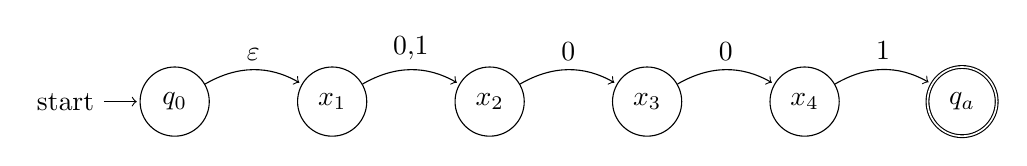
\begin{tikzpicture}[shorten >=1pt,node distance=2cm,on grid,auto] 
   \node[state,initial]   (q_0000)   {$q_0$}; 
   \node[state]           (q_0001) [right=of q_0000] {$x_1$}; 
   \node[state]           (q_0010) [right=of q_0001] {$x_2$}; 
   \node[state]           (q_0011) [right=of q_0010] {$x_3$};
   \node[state]           (q_0100) [right=of q_0011] {$x_4$};
   \node[state,accepting] (q_0101) [right=of q_0100] {$q_a$};
    \path[->] 
    (q_0000) edge[bend left] node {$\varepsilon$}  (q_0001)
    (q_0001) edge[bend left] node {0,1} (q_0010)
    (q_0010) edge[bend left] node {0} (q_0011)
    (q_0011) edge[bend left] node {0} (q_0100)
    (q_0100) edge[bend left] node {1} (q_0101);
\end{tikzpicture}

This takes in as input the bit string representing the assignment of all the variables. Each of the successive nodes
represents the variables, and they transition to the next node on values that would allow the clause to reject.
Notice that since $x_1$ does not appear in the clause, it can take whatever value it wants. So this accepts
the non-satisfying strings ${0,1}001$. 

We can generalize this to more clauses, by making the initial state have $\varepsilon$-transitions 
to a chain for each clause, constructed in the exact same way as the above example. That would
give, with $m$ variables and $c$ clauses, $cm$ nodes. The transition function would take then
$O(cm)$ space to create. This means it can be created in $O(cm)$, or polynomial, time.
This new NFA would accept on any rejecting input since it only takes one failing clause to make the formula
reject. 

If this formula has no accepting input, this NFA would reduce to one that accepts $\{0,1\}^*$, or:

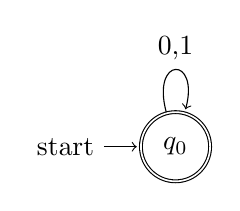
\begin{tikzpicture}[shorten >=1pt,node distance=2cm,on grid,auto] 
   \node[state,initial,accepting] (q_0000)   {$q_0$}; 
    \path[->] 
    (q_0000) edge[loop above] node {0,1} (q_0000);
\end{tikzpicture}

Therefore if we could reduce this NFA in polynomial, we would be able to solve SAT in polynomial time. In other
words we just reduced SAT to minimizing an NFA. Therefore if $P\neq NP$ then there is no polynomial time solution
for this.

\subsection*{Problem 7}




\end{document}




